\documentclass{article}
\usepackage{geometry}
\usepackage{natbib}
\usepackage{amssymb}
\usepackage{amsmath}
\usepackage{graphicx}
\usepackage{hyperref}
\usepackage{textcomp}
\usepackage{array}
\usepackage{booktabs}
\usepackage{makecell}
\usepackage[singlelinecheck=false]{caption}

\geometry{
	a4paper,
	total={170mm,257mm},
	left=30mm,
	top=30mm,
	bottom=20mm,
	right=20mm
}
\title{
	Relatório - Modelagem Matemática\\
	Estudo de População de Aves na Amazônia \\
	\large Usando o Modelo de Reação-Difusçao para avaliar sobrevida de populações em manchas de floresta em áreas desmatadas.
}
\date{2024-07-20}
\author{Paulo Roberto Rodrigues da Silva Filho\\Pedro Paulo Dantas Silva Martins\\Vicente Alves da Silva Sirufo}

\newcommand\R{\mathbb{R}}

\begin{document}
	\renewcommand{\figurename}{Figura}
	\renewcommand{\tablename}{Tabela}
	\renewcommand{\cellalign}{tl}
	\renewcommand{\theadalign}{tl}
	
	\graphicspath{ {./imagens/} }
	\maketitle
	\tableofcontents
	
	\section{Introdução}
	
	\paragraph{}
	Em função do processo de desmatamento da Amazônia, percebeu-se que, dentro das regiões desmatadas, formam-se manchas florestadas isoladas. Tais manchas podem ou não ser adequadas para a sustentação de populações animais. O modelo utilizado para se avaliar a capacidade de tais manchas sustentarem populações é o Modelo de Reação/Difusão, regido pela Equação Diferencial Parcial (EDP) FKPP (Modelo Fischer-Kolmogorov-Petrovsky-Piskunov). Foi avaliada a capacidade de sustentação de população de uma única espécie e, também, de duas espécies em competição.
	
	\paragraph{}
	Para entender o problema, vamos, primeiro, apresentar um diagrama, representando a floresta e áreas desmatadas, conforme pode ser visto na Figura \ref{fig:efloresta}. Conforme essa figura, temos uma grande área de floresta e uma área desmatada que possui manchas de floresta. A área desmatada pode suportar uma população mínima dos animais em estudo, ou suportar uma população temporária de forma que permita a migração dessas populações entre a área de floresta virgem e as manchas na área desmatada.
	
	\paragraph{}
	Uma vez dada essa representação de ambiente, padrão, podemos utilizar o Modelo de Reação-Difusão, assumindo que, entrando uma determinada população em uma mancha de floresta - ou estando essa população lá isolada, antes do processo de desmatamento - há condições de a população se reproduzir dentro dessa área, estando sujeita a restrições do meio, cooperação e competição intra-específica.
	
	\paragraph{}
	Já no caso de duas populações concorrendo na mesma região, devemos também assumir que a região desmatada tenha capacidade de suportar uma quantidade muito baixa dessas populações, de forma que a hipótese da difusão faça sentido. Fazemos, então, uma análise de ambas as populações em conjunto, em competição.
	
	\paragraph{}
	Tanto no caso da população isolada, quanto na de duas populações, a geometria das manchas (tamanho) e características intrínsecas delas permitem definir uma capacidade de carregamento das populações, que afetam as dinâmicas populacionais. A identificação de um tamanho mínimo de mancha e o isolamento dessa mancha em relação à área florestada, ou a outras manchas também são características a relevantes para o estudo do problema.
	
	\begin{figure}[h]
		\centering
		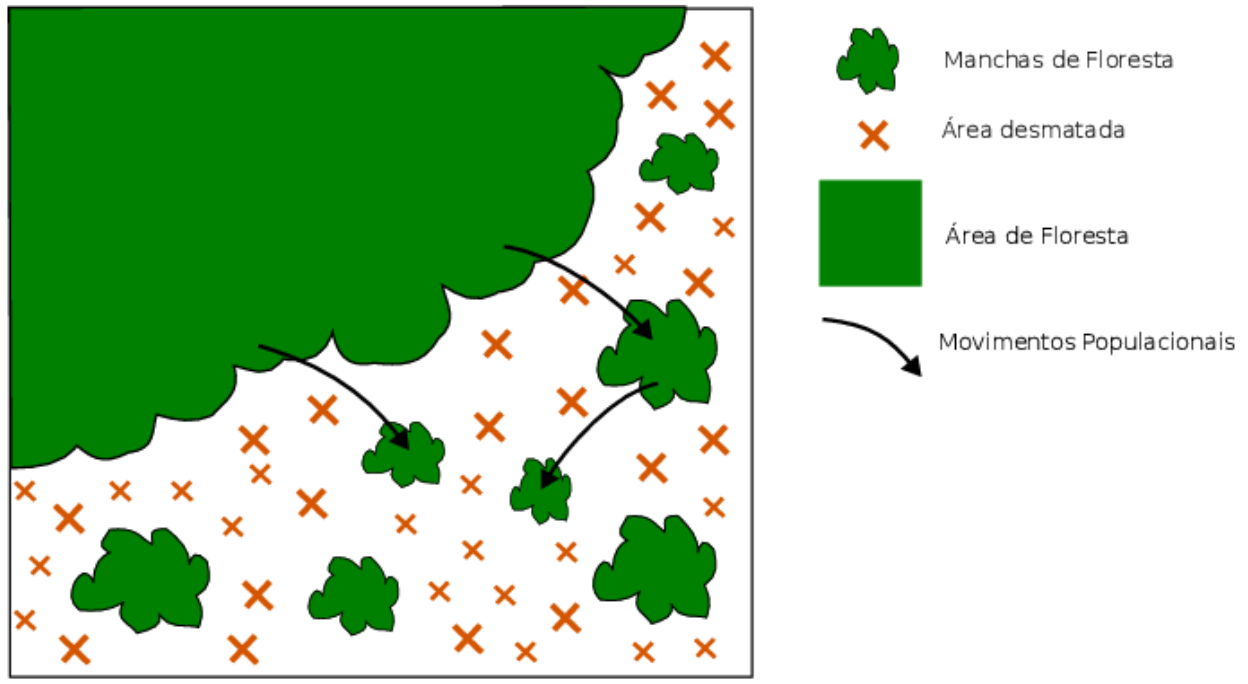
\includegraphics[scale=0.3]{Esquema-Floresta}
		\caption{Representação de área florestada e de manchas de floresta. A área florestada pode ser imaginada como uma mancha de floresta de tamanho infinito, ou, apenas, uma área de tamanho grande o suficiente para ser considerada infinita.}
		\label{fig:efloresta}
	\end{figure}
	
	\section{Modelagem}
	
	\paragraph{}
	Agora vamos apresentar os dois modelos avaliados, o modelo de uma população e o modelo de duas populações. Para ambos os casos são usados variantes da EDP FKPP, apresentadas tais variantes caso a caso.
	
	\subsection{Caso 1: Uma única população}
	
	\paragraph{}
	Para o caso de uma população, o modelo considerado foi FKPP com um termo difusivo (termo de segunda ordem) e os termos reativos, com cooperação (termo linear) e com competição (termo quadrático), sobre uma população $u$:
	
	$$ \frac{\partial u(x,t)}{\partial t} = \alpha u - \beta u^2 + D \frac{\partial^2 u}{\partial x^2}  $$
	
	\paragraph{}
	Com as condições de contorno de Dirichlet:
	
	$$u(x=0,l) = 0 $$
	
	\paragraph{}
	Sendo:
	
	\begin{itemize}
		\item \textbf{u(x,t)}: a população presente na posição espacial e no tempo, na mancha de floresta ou em uma área florestada.
		\item \textbf{D}: taxa de difusividade da população - unidade: \textbf{comprimento\textsuperscript{2}/tempo}.
		\item \textbf{a}: Taxa de cresimento populacional da espécie - unidade: \textbf{1/tempo}
		\item \textbf{b}: Se \textbf{1/C} é a capacidade de carregamento de uma população para uma mancha ou região de floresta, então $C=\frac{b}{a}$, de forma que \textbf{b} indica as condições que atrapalhem o crescimento populacional, como geometria da região de mancha, competição por comida, entre outras.
		\item \textbf{l}: Comprimento (não adimensionalizado) da mancha ou região florestada
	\end{itemize}
	
	\paragraph{}
	Para facilitar a análise, as seguintes transformações são feitas, para se adimensionalizar a equação e, então, avaliar as suas propriedades:
	
	$$ x = x' \sqrt{\frac{D}{a}} $$
	$$ \partial_x = \partial_{x'} \sqrt{\frac{a}{D}} $$
	$$l = L \sqrt{\frac{D}{a}}$$
	$$t = t' \frac{1}{a}$$
	$$\partial_t = \partial_{t'}a$$
	
	\paragraph{}
	Depois, retornando o nome da variável de distância de \textbf{x'} para \textbf{x} e de tempo de \textbf{t'} para \textbf{t}, temos a nova equação:
	
	$$ \frac{\partial u(x,t)}{\partial t} =  \frac{\partial^2 u}{\partial x^2} + u(x,t) - C u^2(x,t)   $$
	
	$$ C(x) =  \begin{cases}
		C_1, & \text{se } |x| < L/2 \\
		C_0, & \text{se } |x| > L/2
	\end{cases}$$
	
	\paragraph{}
	Onde $C_1$ e $C_0$ são a capacidade de carregamento da região interna e externa, respectivamente, de forma que espera-se que a região interna assuma um regime estacionário enquanto a população externa vá assintoticamente para $1/C_0$
	
	\paragraph{}
	Fazemos a seguinte transformação para auxiliar na resolução da EDP:
	
	$$ u = \frac{3}{2} \frac{\phi}{C_1}, $$
	
	$$ \frac{\partial \phi}{\partial t} = \frac{\partial^2\phi }{\partial x^2} + \phi - \frac{3}{2} k*(x)\phi^2 $$
	
	$$ k(x) =  \begin{cases}
		k = \frac{C_0}{C_1}, & \text{se } |x| > L/2 \\
		1, & \text{se } |x| < L/2
	\end{cases}$$
	
	\paragraph{}
	É importante ressaltar que \textbf{k} pode ser interpretado como um indicador do nível de "isolamento" da região interna, como o quão difícil é sair da região ideal ou o quanto a região interna é mais atrativa do que a externa.
	
	\paragraph{}
	Como $\phi$ é uma função contínua e simétrica, e $\frac{2}{3}k$ é uma solução para a parte externa, temos as seguintes condições:
	
	$$\phi_{xx} + \phi - \frac{3}{2}k\phi^2 = 0, \quad x < L/2,$$
	$$\phi_{xx} + \phi - \frac{3}{2}k\phi^2 = 0, \quad 0 > x > -L/2,$$
	$$\phi^o\left(-\frac{L}{2}, \cdot \right) = \phi^i\left(-\frac{L}{2}, \cdot \right),$$
	$$\phi^o_x\left(-\frac{L}{2}, \cdot \right) = \phi^i_x\left(-\frac{L}{2}, \cdot \right),$$
	$$\phi^o(- \infty, \cdot) = \frac{2}{3k}.$$
	
	\paragraph{}
	Onde os índices i/o representam as regiões interna/externa respectivamente.
	
	\paragraph{}
	Resolvendo as equações para vários \textbf{k} e \textbf{L} temos os resultados apresentados nas figuras (...) e (...).
	
	\subsection{Caso 2: Duas populações}
	\paragraph{}
	lalalalala
		
\end{document}
